% !TeX root = main.tex

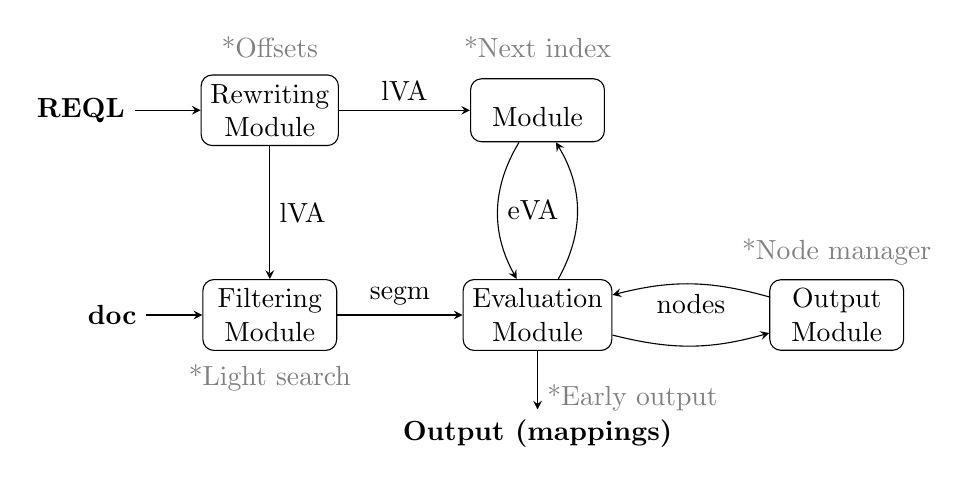
\begin{tikzpicture}[
	every text node part/.style={align=center}]	
	
	\tikzstyle{mmodule}=[rectangle, draw=black, fill=white, minimum height=8mm, minimum width=1.7cm, rounded corners]
	\tikzstyle{medge} = [->,>=stealth,auto]	
	\tikzstyle{opt} = [black!50]
	
	%\draw[step=.5cm, dashed, draw=black!20] (-1,-1) grid (8,3);
	
	\node [mmodule] (rmod) at (1, 2) {Rewriting \\ Module};
	
	\node [mmodule, below of=rmod,node distance=2.6cm] (fmod) {Filtering \\ Module};
	
	\node [mmodule, right of=rmod, node distance=3.4cm] (detmod) {$\cdet$ \\ Module};
	
	\node [mmodule, below of=detmod, node distance=2.6cm] (evalmod) {Evaluation \\ Module};
	
	\node [mmodule, right of=evalmod, node distance=3.8cm] (nodman) {Output \\ Module};
	
	\node[left of=rmod, node distance=2.4cm] (REQL) {\textbf{REQL}};
	
	\node[left of=fmod, node distance=2cm] (doc) {\textbf{doc}};
	
	\node[below of=evalmod, node distance=1.5cm] (output) {\textbf{Output (mappings)}};
	
	\draw[medge] (REQL) edge (rmod); 
	
	\draw[medge] (doc) edge (fmod); 
	
	\draw[medge] (rmod) edge node {lVA} (detmod);
	
	\draw[medge] (rmod) edge node {lVA} (fmod);
	
	\draw[medge] (detmod) edge[bend right] node {eVA} (evalmod);
	\draw[medge] (evalmod) edge[bend right] (detmod);
	
	\draw[medge] (fmod) edge node {segm} (evalmod);
	
	\draw[medge] (nodman) edge[bend right=15] node {nodes} (evalmod);
	\draw[medge] (evalmod) edge[bend right=15] (nodman);
	
	\draw[medge] (evalmod) edge node[opt, pos=0.8] {*Early output} (output); 
	
	\node[opt,above of=rmod, node distance=0.8cm] {*Offsets};
	
	\node[opt,below of=fmod, node distance=0.8cm] {*Light search};
	
	\node[opt,above of=nodman, node distance=0.8cm] {*Node manager};
	
	\node[opt,above of=detmod, node distance=0.8cm] {*Next index};
	
%	\node [state] (n0) at (0,0) {$\bot$};
%	
%	\node [state] (n1) at ($(n0)+(1.3,-1)$) {$[x,\!0$};
%	\node [state] (n2) at ($(n0)+(1.3,0)$) {$[x,\!3$};
%	\node [state] (n3) at ($(n0)+(1.3,1)$) {$[x,\!6$};
%	
%	\node [state] (n9) at ($(n0)+(0,1)$) {$[x,\!9$};
%	
%	\node [state] (n4) at ($(n2)+(1.3,-1)$) {$x\rangle,\!4$};
%	\node [state] (n5) at ($(n2)+(1.3,0)$) {$x\rangle,\!7$};
%	\node [state] (n6) at ($(n2)+(1.3,1)$) {$x\rangle,\!10$};
%	
%	\node [state] (n7) at ($(n4)+(1.3,0)$) {$\cup$};
%	
%	\node [state] (n8) at ($(n7)+(1.3,1)$) {$\cup$};
%	
%	\draw[<-] (n0) to (n1);
%	\draw[<-] (n0) to (n2);
%	\draw[<-] (n0) to (n3);
%	
%	\draw[<-] (n1) to (n4);
%	\draw[<-] (n2) to (n5);
%	\draw[<-] (n3) to (n6);
%	
%	\draw[<-] (n4) to (n7);
%	\draw[<-] (n5) to (n7);
%	
%	\draw[<-] (n7) to (n8);
%	\draw[<-] (n6) to (n8);
%	\draw[<-] (n0) to (n9);

\end{tikzpicture}